\documentclass[11pt, letterpaper]{report}
\usepackage{XL}  % use my awesome template

% \fancyhead[L]{\footnotesize \bfseries Homework 1 \quad \bfseries CS6530 Machine Learning} % set footer
% \fancyfoot[R]{\footnotesize \thepage\ of \pageref{LastPage}} % set footer
\renewcommand{\headrulewidth}{0.0pt} % horizontal line in header
\renewcommand{\footrulewidth}{0.0pt} % horizontal line in footer
\geometry{head=1in, bottom=1in, footskip=25pt} % set margin
\allowdisplaybreaks  % allow cross-page equations


%--------- document starts here -------------------------
\begin{document}

% spacing between equations and text
\setlength{\abovedisplayskip}{3pt}
\setlength{\belowdisplayskip}{3pt}

\thispagestyle{tpstyle} % set the style of title page
{\centering
\vspace*{3.5in}  % force some space
\textbf{\Huge Computational Fluid Dynamics (CFD) with General Equation Mesh Solver (GEMS): A
Tutorial}\vspace{10pt}

\textbf{\Large by Xuxiao Li}\vspace{10pt}

\textit{\large May 3, 2020}
\vspace{8pt}
\centerline{\rule{0.5\linewidth}{0.5pt}}
\vspace{8pt}
\clearpage
\pagenumbering{arabic}  % Number page from the next page
}

\tableofcontents{}

\chapter*{Prologue}
\pagestyle{plain}
In this tutorial, I will cover multiple topics on both the theoretical and practical aspects of
computational fluid dynamics (CFD). With such a rich range of contents in CFD, I will only focus on
the certain methods that I am specialized in, while general concepts will also be discussed. The
major method discussed in this tutorial will be the Finite Volume Method (FVM). FVM is a somewhat
``old school'' method compared to the more recent and advanced variants of the Finite Element Method
(FEM). However, each method has its own advantages and disadvantages when applied to specific
problems. FVM served for a long period of time as the workhorse in solving the fluid mechanics problems, while FEM was
born to solve solid mechanics problems. This is a big gap between the ``fluid'' and the ``solid''
community. Although the trend is to merge the merits from both methods (e.g., discontinuous
Galerkin), but that is still an ongoing research topic and indeed, old habits die hard.
\paraspace

Within the ``fluid'' community, there is a division between those studying compressible flow
problems and those studying incompressible flow problems. Accordingly, the CFD methods can be
divided into the density-based methods (suitable for compressible flow) and pressure-based methods
(suitable for incompressible flow). The major difference here is that the fluid velocity in
compressible flow is typically very large (large Mach number), while fluid velocity is relative
small for incompressible flows. This gap has already been filled through years of efforts.
Density-based methods can also solve incompressible flow problems using the preconditioning
technique, which gives a unified framework for solving fluid dynamics problems. This approach will
be the focus of this tutorial. 
\paraspace

In the 80's, there were several pioneers who contributed significantly to the preconditioning
methods, e.g., Eli Turkel, Bram Van Leer, and Charles Merckle. This tutorial will be focused on
Merckle's preconditioning system, and in fact, the practical part of the tutorial is made based on
one of the in-house codes developed at Merckle's research group. The in-house code is named as the
General Equation Mesh Solver (GEMS) whose main creator is Dr. Ding Li. He worked as a research
associate with Prof. Merckle, initially at the University of Tennessee, and later at Purdue
University. Dr. Li embarked on the development of GEMS about early 1999. In 2002, the version 1.0 is
completed. In 2005, he has added the Maxwell equation into GEMS and also refined multiple features
to improve the generality of the code. In a paper Dr. Li published in 2006, he demonstrated the
capability of GEMS with impressing results.
\paraspace

I feel obliged to mention how I can have the access to the GEMS code. During the time Dr. Ding Li
was at Purdue university, there was a PhD student named Shaoyi Wen who worked with Dr. Li. Shaoyi
was then advised by Prof. Yung Shin whose research group had some collaborations with Prof.
Merckle's group. Shaoyi modified GEMS code for his needs with the help of Dr. Li and published a
paper in 2010 using GEMS to solve thermal-fluid problems in direct laser deposition processes.
Thereafter, the GEMS code seemed to be made available to Prof. Shin's group. Before Shaoyi graduated
from Shin's group, he passed the GEMS code to another PhD student at Shin's group, Wenda Tan. At
this time, Dr. Li has left Purdue (I actually don't know where he went). Wenda has never made
acquaintance with Dr. Li. However, he managed to exploit the GEMS code and have three papers
published in 2013, 2014 and 2015 with it. In these papers, Wenda simulated the laser keyhole welding
processes, and with GEMS, his model incorporated multiple physics and has high fidelity. In 2015,
Wenda ceremoniously graduated from Purdue and became an assistant professor at the University of
Utah. In the fall of 2015, I was registered as a PhD student at the University of Utah and I was
advised by Wenda (Dr. Tan) since then. Therefore, I have the privilege to study the GEMS code and
apply it for my PhD research. I have been exploring the GEMS code since 2017 and still learn new
things about it today. So far I only touched upon the ``basic'' functions in GEMS which is to solve
the basic equations: mass, momentum, energy, and species conservation equations. The unexplored part
is: turbulence modeling and incorporation of Maxwell equations. In the definitive version of the
GEMS, all the equations could be solved and can be customized such that multiple sets of equations
can be assigned to different partitions of the domain. In this tutorial, I will focus on the
``basic'' package which I feel the most comfortable with.  \paraspace

The philosophy of this tutorial will be that more focus is put on the theoretical side. By that I
do not mean that I will linger on derivations of equations, as ``computational'' fluid dynamics
should emphasize on {\bf data structure} and {\bf algorithm} and not on mathematical
reasoning. However, I will not go into details such as ``this subroutine does this'', or ``this
variable is used for this'', or ``how do I output such information''. Instead, I will try to {\bf
speak out} what the code is trying to do, why it should be doing this, and how certain things are
done. With this global picture, you should be able to ``code it up'' by any language, any way you
want. In situations where practical guide is necessary, I will try to separate it by distinct
sections.

\chapter{Mesh}

\section{Definition of Basic Mesh}

The mesh describes the data structure of carrying out CFD simulations. Mesh is a discretization of a
calculation domain (a physical domain in which CFD simulations is conducted). For example, we have a
two-dimensional rectangle in which we want to carry out CFD simulations, as shown in Fig.
\ref{fig-mesh1}a. An exemplary mesh is shown in Fig. \ref{fig-mesh1}b. The rectangle has a width of
2 of a height of 1. The boundary conditions are defined as follows. The left and right edge form
boundary condition batch 1, the top edge is boundary condition batch 2, and the bottom edge is
boundary batch 3. 

\begin{figure}[H]
   \centering
   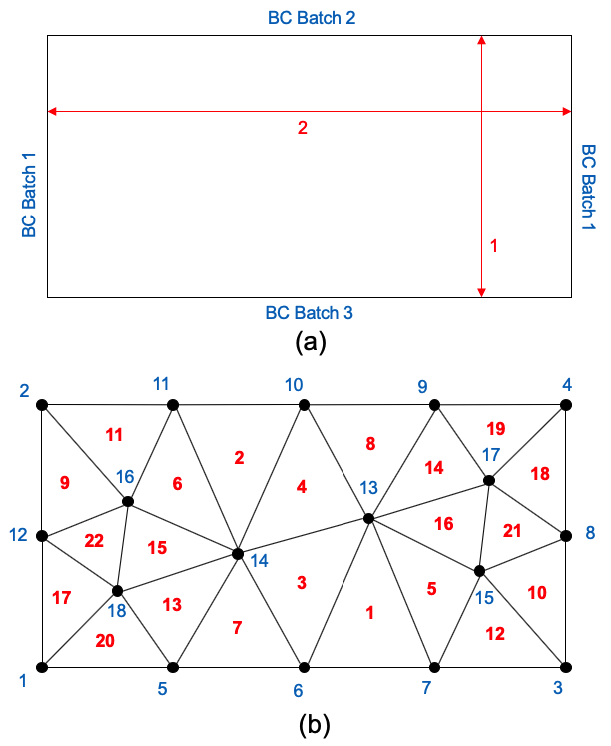
\includegraphics[height=4in]{Mesh1.png}
   \caption{Illustration of mesh. (a) Definition of the calculation domain. (b) A discretization of
   the calculation domain (mesh).}
   \label{fig-mesh1}
\end{figure}

Several notes on defining the calculation domain. First, the dimensions are be scaled up or down
when simulating a particular problem. That is, the numbers of 1 and 2 can mean ``meter'' or
``micrometer'' depending on the specific problem. No need to specify units here. Second, the
boundary conditions must be carefully stated. We need to first think about how many distinct BC's we
want to define. Then we assign each distinct BC (BC batch) to a segment of the domain boundary. Here,
we have three unique BC's. Each of them is assigned with a certain segment of the domain boundary.
\paraspace

After the calculation domain is defined. We seed the domain with a set of points (black circles in
Fig. \ref{fig-mesh1}b) in the domain, referred to as the ``{\bf nodes}''. The nodes are indexed by
the blue numbers. We have 18 nodes in the domain. Next, we connect the nodes to form a
``tessellation'' of the domain. Here we use all triangles. In general, there is a large flexibility
of the tessellation. You can use triangles, polygons, or their mixture in two-dimension. In
three-dimension, there are the tetrahedral, pyramid, prism, and hexagon, or their mixture (called
hybrid mesh). This flexibility is incorporated in the GEMS code, therefore the name ``General
Equation Mesh Solver''.  Now with the tessellation, we divide the domain into triangular
``elements'', from which the name ``Finite Element Method'' is originated. However, we will only
focus on the Finite Volume Method in this document, and the elements will be referred to as the
``{\bf cells}''. We have 22 cells in the domain and they are indexed with the red numbers. It should
be mentioned that the indexing of the nodes and cells does not matter in the definition of the mesh.
\paraspace

Now we can define the ``{\bf cell-node connectivity}'' by associating cells with its corresponding
nodes. For example:
\begin{verbatim}
   cell 1 ---> node 6, 7, 13
   cell 2 ---> node 11, 10, 14
   ...
\end{verbatim}
With that, let's design the following data structures \verb+cell+ and \verb+node+ to better
represent this information. For \verb+node+, we have (in Fortran):

\begin{lstlisting}{language=[90]Fortran}
   type node
      real :: xyz(ndim)
   end type node
\end{lstlisting}

where \verb+ndim+ is the number of dimensions and \verb+xyz+ is the coordinate of the node. We will
need to have an array of nodes \verb+nodes(:)+ to store all the information about nodes. For cells,
we have the following data type:

\begin{lstlisting}{language=[90]Fortran}
   type cell
      real :: centp(ndim)
      integer, pointer :: c2n(:)
   end type cell
\end{lstlisting}

where \verb+centp+ is the centroid of the cell and \verb+c2n+ is the node indices associated with
this cell. Note that we can calculate the centroid of the cell based on the nodal coordinates
associated with the cell. We will also need an array of cells \verb+cells(:)+ to store all the
information about cells. Now we have introduced two important data types \verb+node+ and
\verb+cell+. Each of these data types can have more attributes which we will build on later.
\paraspace

Now we still need to add the last part of the mesh definition, the boundary conditions. To define
the boundary conditions of the mesh, we have to introduce another important concept, ``{\bf
faces}''. Faces are the edges (or facets in 3D) that form the boundary of a cell. There are three
faces per one triangle cell, and six faces per one hexagon cell (in 3D), etc. Faces that are shared between
two cells are defined as {\bf interior faces}. Faces that are only belong to a single cell are
defined as {\bf boundary faces}. Faces can be distinguished by a set of nodes, which brings about
the ``face-node'' connectivity. We will discuss in further details about faces in the next section.
For now, we use face to define the boundary conditions as follows:
\begin{verbatim}
   BC batch 1 ---> 4 faces: (1, 12), (2, 12), (3, 6), (4, 8)
   BC batch 2 ---> 4 faces: (2, 11), (11, 10), (10, 9), (9, 4)
   BC batch 3 ---> 4 faces: (1, 5), (5, 6), (6, 7), (7, 3)
\end{verbatim}
That is, we use the boundary faces (shown as node sets above) to define the segments of boundaries.
Each set of faces represents a unique BC. It is convenient to create a data type for the BC's:

\begin{lstlisting}{language=[90]Fortran}
   type bc_type
      integer :: label
      integer :: igrp
      integer :: itype
   end type bc_type
\end{lstlisting}

Here, \verb+label+ is a distinct integer to indicate the batch of BC. \verb+igrp+ indicates which
``group'' of BC it is. In GEMS, there are 6 groups of BC's: 

\begin{itemize}
   \item Group 1, Inlet
   \item Group 2, Outlet
   \item Group 3, Farfield
   \item Group 4, Wall
   \item Group 5, Geometric (e.g., symmetric, periodic)
   \item Group 6, MHD (for Maxwell equations)
\end{itemize}

Each group of BC can have sub-categories (types) which is saved in the attribute \verb+itype+.
Again, we need an array of BC's \verb+bc(:)+ to store all the information. Apparently, the
association between BC and faces should be defined based on the face lists of each batch of BC,
which will be discussed in the next section.
\paraspace

So far, we have introduced the complete information to define a mesh, summarized as follows:

\begin{enumerate}
   \item Nodal coordinates.
   \item Cell-node connectivity.
   \item Face list in each BC batch.
\end{enumerate}

We emphasize this contains the complete information of a mesh. We refer this piece of information as
the ``basic mesh'' or the finite element mesh. The information is complete but is not organized in a
way convenient for finite volume method. As we will see, additional data types can be constructed
based on the basic mesh and be used to facilitate finite-volume computation. 
\paraspace

\section{Finite Volume Mesh}

We establish the data type \verb+face+ from the basic mesh to form the ``finite volume mesh''. The
\verb+face+ type has much more emphasis in the finite volume method as the fluxes on the faces need
to be computed. On the opposite side, the finite element method emphasize on the data type
\verb+node+. The \verb+face+ type is defined as:

\begin{lstlisting}{language=[90]Fortran}
   type face
      integer :: itype
      type(cell), pointer :: left_cell
      type(cell), pointer :: right_cell
      integer, pointer :: f2n(:)
      real :: centp(ndim)
   end type face
\end{lstlisting}

Here, \verb+itype+ defines the type of the face which we will elaborate later. The pointers
\verb+left_cell+ and \verb+right_cell+ refers to the two cells that share this face. This is
referred to as the {\bf face-cell connectivity}. The pointer \verb+f2n(:)+, like \verb+c2n(:)+, is
the {\bf face-node connectivity}, which refers to the set of nodes that defines the face. At last,
the center of the face \verb+centp+ can be calculated based on the nodal coordinates which can be
found through \verb+f2n(:)+. The \verb+face+ type constructed based on Fig. \ref{fig-mesh1}b is
shown in Fig. \ref{fig-mesh2}. The faces are indexed with the green number and there are 39 faces in
the calculation domain.

\begin{figure}[H]
   \centering
   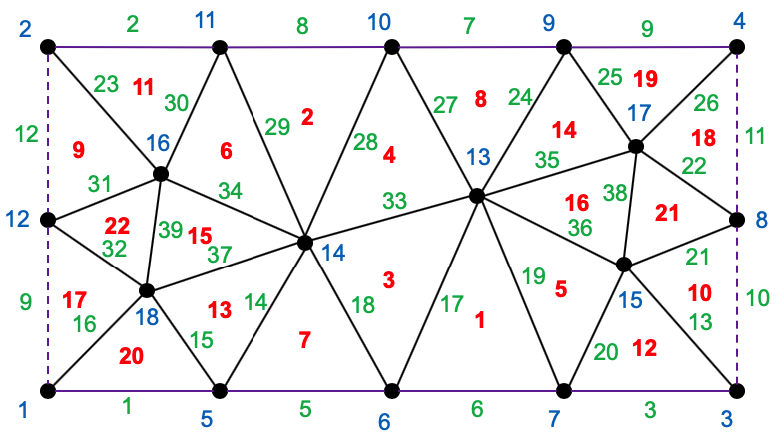
\includegraphics[height=3in]{Mesh2.png}
   \caption{Construction of faces to make the finite volume mesh.}
   \label{fig-mesh2}
\end{figure}
\paraspace

How to collect all the face information from the basic mesh? The face information can be found from
the cell-node connectivity. For example:

\begin{verbatim}
   cell 1 ---> node 6, 7, 13, we can find:
      face 1 --> node 6, 7
      face 2 --> node 7, 13
      face 3 --> node 13, 6
   cell 2 ---> node 11, 10, 14, we can find:
      face 4 --> node 11, 10
      ...
\end{verbatim}

By doing so we obtain an array of faces, \verb+faces(:)+. Two points need to be noted. First, the
face-node connectivity is contained in the cell-node connectivity, but we still need to know which
nodes in a cell can form a face. If all cells are triangles, any combination of the three nodes of
the cell will form a face. But for quadrilaterals and 3D cells, a set of rules need to be
pre-defined to help extracting the face-node connectivity.  The second note is, faces identified
this way will be double-counted. We need to delete the repeating faces. This can be done by checking
whether the face-node connectivity \verb+f2n+ is repeating. In doing so, every time we find a
repeating face, it means two cells share the same face.  Therefore, the \verb+left_cell+ and the
\verb+right_cell+ can be found. We note that the ``left'' and ``right'' do not mean the literal
directions. In practice, we always make the cell with the smaller index (red number in Fig.
\ref{fig-mesh2}) to be the left cell and the other cell to be the right cell.
\paraspace

There are some faces that are only belong to a single cell. These faces are referred to as the
``{\bf boundary faces}'' (face 1 - 12 in Fig. \ref{fig-mesh2}). Boundary faces are regarded as
special faces and we will make them to be at the front of \verb+faces(:)+ by {\bf swapping faces} in the
face array. We assign the only cell
that a boundary face is associated to be the {\bf left cell} of the boundary face. That is, the
boundary faces only have \verb+left_cell+ which is the interior cell, for now.
\paraspace

In CFD computation, it is required that every face be associated with two cells, including the
boundary faces. Therefore, we need to create a ``{\bf ghost cell}'' as the right cell for the
boundary faces. Ghost is an overused word (but I still sometimes use it). The ghost cell is
alternatively referred to as the ``{\bf boundary cell}''. To create the ghost cells, we can simply
mirror the interior cell with respect to the boundary face. However, there is one exception, the
periodic boundary condition. For periodic BC, we need to translate the same cell ``on the other
side'' to form the ghost cell. To illustrate, the boundary faces are marked purple in Fig.
\ref{fig-mesh2}. We let BC batch 1 to be the periodic BC, and the periodic boundary faces are marked
as dashed purple. To create the boundary cells, we can mirror cell 11, 2, 8, 9, 20, 7, 1, and 12 for
face 2, 8, 7, 9, 1, 5, 6,  3, respectively. For periodic boundary cells, we need to translate cell
9, 17, 18, 10 for face 11, 10, 12, 9, respectively. This indicates that the periodic boundary faces
must ``match'', otherwise, the mesh is ill-defined for the periodic BC. The periodic boundary faces
are special boundary faces. We will move these faces to the end of the boundary faces. That is,
\verb+face(1)+ to \verb+face(12)+ are the boundary faces, and \verb+face(9)+ to \verb+face(12)+ are
reserved for periodic boundary faces.  We will dedicate an entire section to periodic BC later.
\paraspace

One last note about face types. The interior faces (black solid line in Fig. \ref{fig-mesh2}) has
\verb+itype = 0+. The boundary faces has a positive \verb+itype+ which equals to the index in
\verb+bc(:)+ that the boundary face is associated with. For example, we have 3 batches of BC's, and
we create an array \verb+bc(:)+ with a length of 3. Each element in \verb+bc+ corresponds to one
specific BC batch. Say, batch 1 corresponds to \verb+bc(3)+. Then the \verb+itype+ for face 9, 10, 11,
12 will be equal to 3. There can be other \verb+itypes+ which we shall discuss later.
\paraspace

To summarize, the finite volume mesh consists of the following information:
\begin{enumerate}
   \item Nodal coordinates.
   \item Cell-node connectivity.
   \item Face types, face-cell connectivity and face-node connectivity.
\end{enumerate}
Notice that the information about BC's can be fully described by the \verb+bc(:)+ array and the
\verb+itype+ in \verb+face+.
\paraspace

\section{Partitioning of Mesh}

Now we have got a finite volume mesh, with three essential data types, \verb+node+, \verb+cell+, and
\verb+face+. It is no problem to plug this mesh into some CFD code. However, today's computation
lives in a parallel world. Any practical CFD code must enable parallel computing. GEMS uses MPI
for parallel computing. In MPI, the finite volume mesh is decomposed into partitions. Each partition
is assigned to one ``core'' (or one CPU, one ``processing element'', any way you want to call it).
Each core only has information about its own partition of the entire domain and has no idea of what the
entire domain is like. Such a partitioning is shown in Fig. \ref{fig-mesh3}.

\begin{figure}[H]
   \centering
   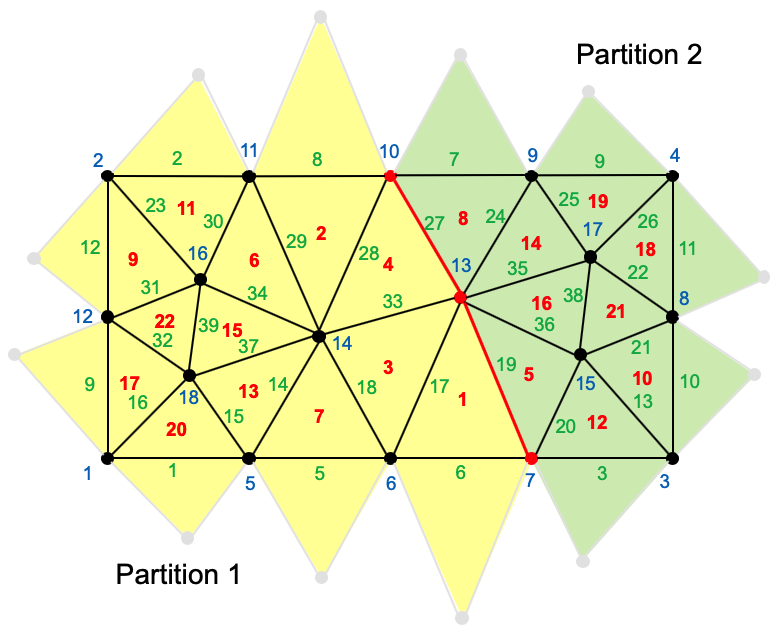
\includegraphics[height=4in]{Mesh3.png}
   \caption{Partitioning of calculation domain}
   \label{fig-mesh3}
\end{figure}

Here the contour formed by the solid black line is the calculation domain, including the nodes
(indexed by blue), cells (indexed by red) and faces (indexed by green). We also show the ghost cells
(boundary cells) marked by the gray lines. It is noted that the ghost cells can be entirely derived
from the boundary faces and need not be store prior to CFD simulation. Based on this configuration,
we partition the domain into two partitions. First, we identify which {\bf cells} belong to which
partition. Then the nodes and faces shared by cells from both partitions can be identified (marked
by red). These delineates the {\bf interface} of the partitions. The nodes, cells, and faces belong
to partition 1 is shadowed by yellow and those belong to partition 2 is shadowed by green.
\paraspace

Now we split the domain into two partitions as shown in Fig. \ref{fig-mesh4}. Take partition 1 for
example, the nodes, cells, and faces all need to be re-indexed as partition 1 does not have any
information about partition 2. The re-indexed numbers are shown by the corresponding blue, red and
green numbers. For partition 1, to establish the ``communication'' with the external world (which
means partition 2 in this case), we identify all the cells (including ghost cells) in partition 2
that shared nodes with partition 1. Those are the orange-shaded cells indexed from 1 - 7. This means
there are 7 cells we need to create in partition 1 as ``containers'' to receive the information from
partition 2. Same for partition 2, we need to create 6 ``container'' cells to receive information
from partition 1. From a global point of view (Fig. \ref{fig-mesh3}), the container cells
(orange-shaded cells in Fig. \ref{fig-mesh4}) for both partitions can be identified. Then, we can
correspondingly mark in each partitions the cells that need to be ``sent'' out to the external
world (the sky-blue shaded cells in Fig. \ref{fig-mesh4}). Note that the ``sending cells'' and the
``receiving cells'' must match. That is, the receiving cells in partition 1 (orange) must be match
the sending cells in partition 2 (sky-blue), and vice versa.

\begin{figure}[H]
   \centering
   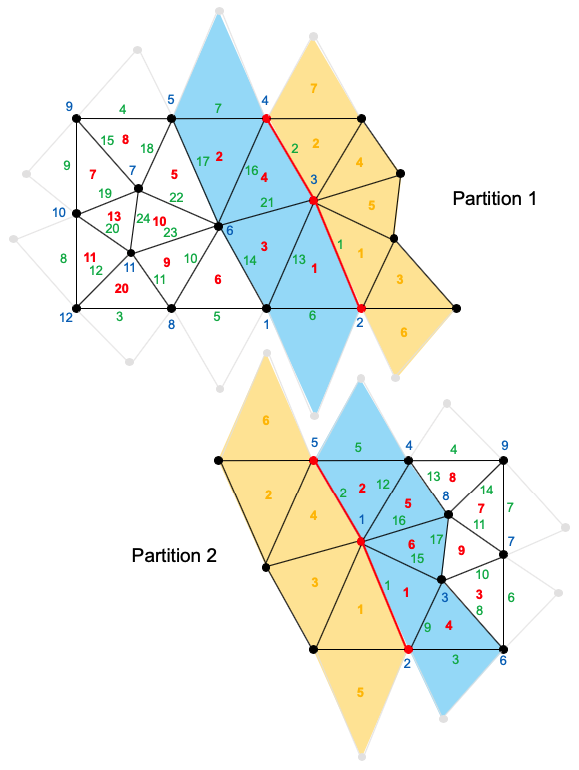
\includegraphics[height=6in]{Mesh4.png}
   \caption{Splitting of the domain and re-indexing.}
   \label{fig-mesh4}
\end{figure}
\paraspace

To represent the data structure for communication among partitions, in GEMS, the data type
\verb+itf+ (standing for ``interface'') is created: 

\begin{lstlisting}{language=[90]Fortran}
   type itf
      integer :: nn
      integer, pointer :: np(:), nnp(:)
      type(cell), pointer :: pcell(:) 
   end itf
\end{lstlisting}

where \verb+nn+ is the number of partitions from which the current partition receives data; \verb+np+
and \verb+nnp+ are arrays with a length of \verb+nn+. \verb+np+ stores the id of the partitions from
which the current partition receives data, and \verb+nnp+ stores the number of cells to receive from
each partition. Finally, \verb+pcell+ is the array of ``container'' cells to store the received
data. \verb+pcell(:)+ should have a length of \verb+sum(nnp)+. It should be noted that the
\verb+pcell(:)+ array needs to be {\bf allocated} as it is ghost cells that do not exist in the
physical domain of partition 1. 
\paraspace

So far, the attributes of \verb+itf+ are only relative to receiving (orange-shaded cells in Fig. \ref{fig-mesh4}). We need to add similar attributes for sending:

\begin{lstlisting}{language=[90]Fortran}
   type itf
      ...
      integer :: nc
      integer :: cp(:), ncp(:)
      type(neighbour_cell), pointer :: scell(:)
   end type itf
\end{lstlisting}

Here \verb+nc+ is the number to partitions to which the current partition needs to send data;
\verb+cp+ is the id's of partitions to which the current partition sends data and \verb+ncp+ is the
number of cells to send to each partition in \verb+cp+. The array \verb+scell(:)+ points to the
cells in the current partition whose information will be sent to external partitions. Notice that
instead of using \verb+type(cell)+, we invented a new data type \verb+neighbour_cell+ for
\verb+scell(:)+. This data type is a {\bf nested type} for the type \verb+cell+:

\begin{lstlisting}{language=[90]Fortran}
   type neighbour_cell
      type(cell), pointer :: to_cell
   end type neighbour_cell
\end{lstlisting}

There is nothing in the type \verb+neighbour_cell+ but a \verb+cell+ pointer. This nested structure
is adopted in GEMS to represent that the cell pointer {\bf needs not be allocated}. Rather, it is
merely a reference to cells already allocated.
\paraspace

How can we construct such data type \verb+itf+? It must start from the global domain (Fig.
\ref{fig-mesh3}). First we identify the container cells for each partition (1 \& 2). Then we can
identify the sending cells in partition 1 based on the container cell in partition 2, and we record
the cell id's and boundary face id's (for boundary cells to send). Same for partition 2. For
container cells, they don't yet exist in each partition. Therefore, (for example, in partition 1), we simply
allocate 7 ``empty'' cells. The empty cells will be fulfilled once the data is received from
partition 2.
\paraspace

Although the container cells are empty, the cell-node and cell-face connectivity between the
container cells and the nodes and faces needs to be identified. Take partition 1 for example, for
cell-node connectivity, we need to record in each container cell which node index in partition 1 it
is associated with. Note, only record those nodes in partition 1, so we have 2 nodes for
\verb+pcell(1:2)+ and only 1 node for \verb+pcell(3:7)+. For face-cell connectivity, we need to
associate the \verb+right_cell+ of \verb+faces(1:2)+ with \verb+pcell(1:2)+ for partition 1. For
partition 2, we associate the \verb+right_cell+ of \verb+faces(1:2)+ with \verb+pcell(1)+ and
\verb+pcell(4)+. The \verb+left_cell+ will be assigned to the other cell which is interior cell. It
should be mentioned that the \verb+left_cell+ of a face always belong to the interior of the domain.
\paraspace

The indexing convention for the partitioning is as follows. We first index interior cells for
\verb+pcell+ and then the boundary cells. Same for the \verb+scell(:)+. Note, the indexing of
\verb+scell(:)+ and \verb+pcell(:)+ must match across partitions. The faces that has a
\verb+right_cell+ as a container cell are referred to as the ``{\bf partitioning faces}'' and are
considered as another type of special faces. A special (large) number is reserved for the
\verb+itype+ of the partitioning faces, 19621011. The partitioning faces are indexed from very
beginning of the \verb+faces+ array (by proper face swapping). Therefore, we have a rather complex
rule for face indexing (take partition 1 as example):

\begin{enumerate}
   \item Index partitioning faces (face 1 \& 2), \verb+itype = 19621011+
   \item Index boundary faces that are not periodic boundaries (face 3 - 7), \verb+itype = + positive
      number (from one to the number of BC's)
   \item Index periodic boundary faces (face 8 \& 9), \verb+itype = + the number for periodic BC
   \item Index interior faces (face 10 - 23) , \verb+itype = 0+
\end{enumerate}

Also, we record the number of partitioning faces in the type \verb+itf+ by adding the variable
\verb+nitf+:

\begin{lstlisting}{language=[90]Fortran}
   type itf
      ...
      integer :: nitf
   end type itf
\end{lstlisting}
\paraspace

With the mesh partitioning, we will generate sepearate mesh files for each partition. Let us now
summarize the information contained in each mesh file:

\begin{enumerate}
   \item Nodal coordinates for current partition
   \item Cell-node connectivity for current partition
   \item Face-cell connectivity, face-node connectivity as well as face type for current partition
   \item Sending information: No. of sending-to partitions, No. of total sending cells. For each
      sending-to partition,
      \begin{enumerate}
         \item sending-to partition id, No. of to-be-sent iterior cells, No. of to-be-sent boundary cells
         \item for to-be-sent iterior cells, store those cell id
         \item for to-be-sent boundary cells, store those boundary face id
      \end{enumerate}
   \item Receiving information: No. of receive-from partitions, No. of total receiving (container)
      cells. For each receive-from partition, 
      \begin{enumerate}
         \item receive-from partition id, No. of container cells to receive from this partition
         \item for each container cell, record the node shared between container cell and the
            current partition
      \end{enumerate}
\end{enumerate}
\paraspace

\section{Periodic Boundary Condition}

The treatment of periodic BC deserves a separate section to describe. The difficulty in treating
periodic BC arises when information in the boundary cells for periodic BC cannot be directly
obtained from the left cell of the boundary face (i.e., mirroring). Rather, we need to find the left
cell of the matching boundary face ``on the other side''. Moreover, when the domain is partitioned,
the matching face may not even exist in the current partition, and communication must be established
specially for treating periodic BC.
\paraspace

To better illustrate the treatment of periodic BC, we modified the original definition of BC's in
Fig. \ref{fig-mesh1}. As shown in Fig. \ref{fig-mesh5}a, we define only two batches of BC's and both of them are
assigned to be periodic BC's. Each batch consists of a pair of walls. The corresponding mesh (before
partition) is shown in Fig. \ref{fig-mesh5}b. We emphasize again that boundary faces in the mesh for periodic BC
must ``match'', i.e., sharing the exact same nodal coordinates in all directions excluding the
periodic direction. Otherwise, the face meshing is ill-defined for the periodic BC.

\begin{figure}[H]
   \centering
   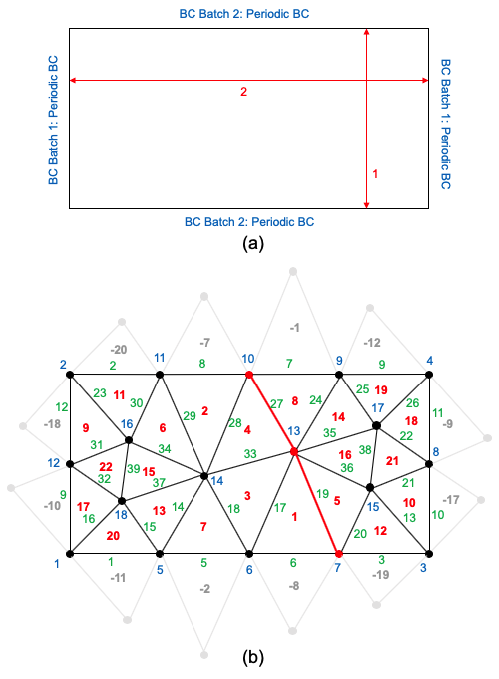
\includegraphics[height=5in]{Mesh5.png}
   \caption{Re-define the boundary conditions. (a) Set two pairs of walls as 2 batches of periodic
   BC. (b) The mesh corresponding to the setup in (a).}
   \label{fig-mesh5}
\end{figure}
\paraspace

In Fig. \ref{fig-mesh5}b, again, the node, cells, and faces of the global domain are indexed. The
global domain will be partitioned into two parts as separated by the red line like before. The
boundary cells are marked by the gray edges. The first step to construct periodic BC is to find the
``matching cells'' for the boundary cells. This step is shown with the global indices in Fig.
\ref{fig-mesh5}b. We index the periodic boundary cells by a negative number whose absolute value
matches the global indices of the matching interior cells, as shown in Fig. \ref{fig-mesh5}b. After
the matching cells are found (globally), we merge the two (or more) batches of periodic BC as one
batch. This is due to the special treatment of periodic BC in GEMS. As long as matching cells are
found, the complete information regarding to all periodic BC's is known. Therefore, they are viewed
as a single package (of BC) in GEMS.  \paraspace

Now, let's illustrate the specific data structure of periodic BC by considering the partitioning
layout shown in Fig. \ref{fig-mesh6}. Take partition 1 for example, the yellow region is the
physical domain of partition 1 and the orange region is the container cells to receive information
from partition 2, like before. There are 7 container cells, as indexed by the orange numbers. Now,
the periodic boundary cells are considered as a second type of container cells, as indexed by the
purple numbers. There are 8 {\bf periodic container cells} and they are indexed as negative number to
differentiate with the ``partitioning container cells''. It is noted that some of these periodic
container cells needs to be received from partition 2 (-4, -6 and -7), but some of them are actually
just the interior cells
in partition 1 but ``on the other side'' of the boundary faces of -2, -5, -1, -3. GEMS will treat all
the periodic container/boundary cells by communications between partitions, in a unified manner. For
cell -2, -5, -1 and -3, they will be communicated from partition 1 and to partition 1. This is the
difference between communicating partitioning cells and periodic boundary cells. The latter involves
communicating with the partition itself (totally OK in MPI).

\begin{figure}[H]
   \centering
   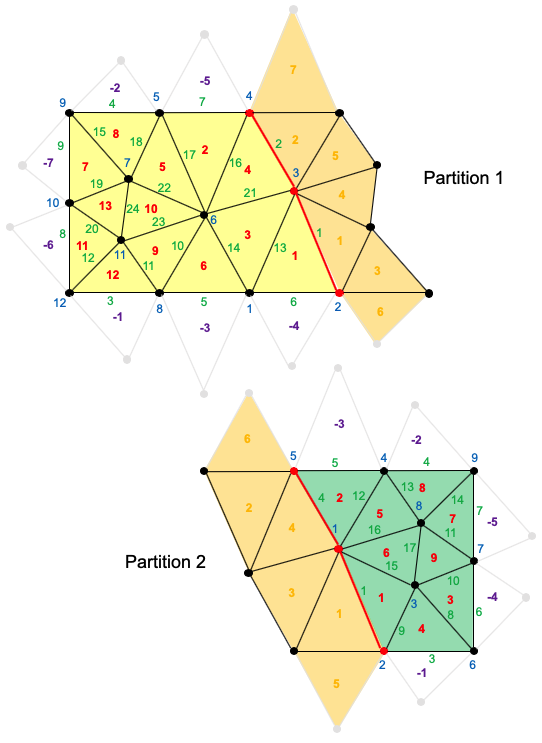
\includegraphics[height=6in]{Mesh6.png}
   \caption{Demonstration of the treatment of periodic BC.}
   \label{fig-mesh6}
\end{figure}
\paraspace

If we examine on the interior cells in Fig. \ref{fig-mesh5}b, each interior cell belongs to a
unique partition (separated by the red line). Also, with the matching cell known for each
periodic boundary face, we can know from where the periodic container cells should receive.
The exact same data structure \verb+itf+ as in partitioning communication is used to represent
the communication for periodic BC. \verb+pinterf+ (of the type \verb+itf+) can be constructed in both
partitions in the following way:

\begin{verbatim}
   pinterf of Partition 1:
      2 receiving batches:
      receive-from id ---> 1 (itself) and 2
      No. of container cells ---> 4 (from id = 1) and 3 (from id = 2)
      periodic boundary faces to bear the container cells:
         face 4, 7, 3, 5 for from id = 1
         face 8, 9, 6 for from id = 2

      2 sending batches:
      sending-to id ---> 1 (itself) and 2
      No. of to-be-sent cells ---> 4 (to id = 1) and 3 (to id = 2)
      To-be-sent iterior cell indices:
         cell 8, 2, 6, 11 for to id = 1
         cell 7, 11, 1 for to id = 2
   end pinterf

   pinterf of Partition 2:
      2 receiving batches:
      receive-from id ---> 1 and 2 (itself)
      No. of container cells ---> 3 (from id = 1) and 2 (from id = 2)
      periodic boundary faces to bear the container cells:
         face 4, 5, 3 for from id = 1
         face 6, 7 for from id = 2

      2 sending batches:
      sending-to-id ---> 1 and 2 (itself)
      No. of to-be-sent cells ---> 3 (to id = 1) and 2 (to id = 2)
      To-be-sent iterior cell indices:
         cell 2, 7, 3 for to id = 1
         cell 8, 4 for to id = 2
   end pinterf
\end{verbatim}

In constructing the above data structure, we first identify the container cells in both partitions.
These are ``ghost cells'' to be allocated and are not interior cells in the domain. Then, the
sending cells (interior cells) are determined based on the container cells in each partition. It is
noted that for periodic boundary cells, we do not need the cell-node connectivity as in partitioning
cells. We only need the cell-face connectivity. We associate periodic boundary faces with their
corresponding container cells. Then, the cell-node connectivity of the container cells is equivalent
to the face-node connectivity of the periodic boundary faces. This can be applied to other type of
boundary cells. The cell-node connectivity of boundary cells will always be equivalent to the
face-node connectivity of the corresponding boundary faces.
\paraspace

As a final note, the communication of periodic BC must precede the communication of the
partitioning. This is because we periodic BC communication will first fill in all the boundary
cells, some of which can then be sent out via the partitioning communication.
\paraspace

\section{Practical Guide}

\chapter{Fundamentals of Fluid Mechanics}

\section{Governing Equations}

\section{Thermodynamic Relations}

\section{Matrix Representation}

\section{Preconditioning: Motivation}

\chapter{Algorithm}

\section{Spatial and Temporal Discretization}

\section{Preconditioning: Implementation}

\section{Gradient Computation}

\section{Construction of Flux Function}

\section{Solving Linear Systems}

\section{Boundary Conditions}

\chapter{Benchmark Tests}

\section{One-Dimensional Euler Equation}

\section{Propagation of Vortex}

\section{Flow Around a Cylinder}

\section{Decay of Isotropic Turbulence*}

\chapter{Awkward Level-Set GEMS}

\section{The Level-Set Function}

\section{Hamilton-Jacobi Equations}

\section{Ghost Fluid Method}

\section{Lagrangian Particle Tracking*}











\clearpage
\bibliographystyle{IEEEtran}
\bibliography{./ref.bib}
\end{document}





